\documentclass[journal]{IEEEtran}

\usepackage{graphicx}
\usepackage{caption}
\usepackage{subcaption}
\usepackage{amssymb}
\usepackage{relsize}
\usepackage{array}
\usepackage{tikz}
\usepackage{adjustbox}
\usepackage{multicol}

\ifCLASSINFOpdf
\else
\fi


% *** SPECIALIZED LIST PACKAGES ***
\hyphenation{op-tical net-works semi-conduc-tor}


\begin{document}

\title{Transformers for Electricity Price Forecasting}


\author{Oscar~Llorente,
        Jose~Portela,
\thanks{O.Llorente is with Ericsson, e-mail: oscar.llorente.gonzalez@ericsson.com.}% <-this % stops a space
\thanks{J. Doe and J. Doe are with Anonymous University.}% <-this % stops a space
\thanks{Manuscript received April 19, 2005; revised August 26, 2015.}}



% The paper headers
\markboth{Journal of \LaTeX\ Class Files,~Vol.~14, No.~8, August~2015}%
{Shell \MakeLowercase{\textit{et al.}}: Transformers for Electricity Price Forecasting}




% make the title area
\maketitle

% As a general rule, do not put math, special symbols or citations
% in the abstract or keywords.
\begin{abstract}
The abstract goes here.
\end{abstract}

% Note that keywords are not normally used for peerreview papers.
\begin{IEEEkeywords}
IEEE, IEEEtran, journal, \LaTeX, paper, template.
\end{IEEEkeywords}

\IEEEpeerreviewmaketitle



\section{Introduction}

\section{Attention in Deep Learning}
This section will show the evolution of Attention mechanisms throughout time, starting in the NLP field where they were created.

There are many problems in Artificial Intelligence, as classification based on features, that do not need any temporal notion. In the field of Deep Learning the same happens. An example in this area would be Image Classification or Image Segmentation. However, there are other areas, as NLP, where this type of knowledge is needed. In language the order of words matters. For this reason from the beginning the field has used a different type of algorithms than Computer Vision. The first deep learning approach was Recurrent Neural Networks~\cite{rumelhartLearningInternalRepresentations1987}. This type of Neural Network ha a structure that allows it to remember information of past events. Theoretically, this type of Neural Networks is able to learn very long term dependencies, something fundamental for NLP. However, in practice this is not the case, as explored in~\cite{bengioLearningLongtermDependencies1994}. For solving these, another variant from RNNs was created: Long Short Term Memory Networks~\cite{hochreiterLongShortTermMemory1997}.

One of the main problems approached by the NLP community is translation.
This is a problem of sequence to sequence type, where the output is not only a label, as in Image or Text Classification, but a multiple output, in this case a complete sentence. Another example in NLP domain would be Question Answering. For this type of problems in NLP is used a structure of encoder-decoder. To improve the encoder-decoder architecture explained before, another type of layer was presented, an Attention layer~\cite{bahdanauNeuralMachineTranslation2016}. This layer is, in fact, the basis of the Transformer model. The Attention layer allows the decoder to focus its attention in a specific word or group of words from the input of the encoder (the original sentence in the case of translation). This helped improved the State of the Art of many NLP problems. However, in 2017, Google developed a model based only on the Attention layer, without any Recurrent layer, the Transformer.

One of the advantages of the Transformer architecture is that it enables the generation of much bigger Deep Learning models. An example of this would be the BERT model~\cite{chenEvaluatingLargeLanguage2021}, used for many purposes by retraining it with new data. There
is, in fact, an entire python library dedicated to this purpose which is used widely
called transformers. Then, in recent years, extraordinarily large models that have
accomplished really difficult tasks, like generating very realistic stories (GPT3)~\cite{brownLanguageModelsAre2020}
or even writing programming code (Codex)~\cite{chenEvaluatingLargeLanguage2021}, were created.
Beside the NLP domain, where the effectiveness of the Transformer is undeniable, recently the Transformer architecture has achieved great success in other areas, as Autonomous Vehicles~\cite{teslaTeslaAIDay2021} or Image Classification~\cite{dosovitskiyImageWorth16x162022}. This is, as mentioned before, one of the main reasons that motivates this article because it proofs
that this type of model can be used in other areas successfully. As an example of how other data can be treated as words to use a Transformer one can look into the structure of Vision Transformer (ViT), the Transformer applied to Image Classification.

\section{Proposed Transformer model for Electricity Price}
In this section the model proposed will be explained. Here the structure proposed is based on a Transformer Encoder only, as in the case of BERT~\cite{devlinBERTPretrainingDeep2019} or ViT~\cite{dosovitskiyImageWorth16x162022}. 

First, it is important to take into account that the model has two different sources of data, the prices and the exogenous variables. Therefore, some modifications to the encoder architecture have been made to include that. The architecture can be observed in Figure~\ref{fig: model architecture}.

The model has four main structures, two types of Embeddings, a stack of Transformer Encoder and a final Multi-Layer Perceptron for making the final predictions. Due to the importance of the Transformer Encoder, it can also be observed the structure of it in Figure~\ref{fig: encoder architecture}.

\begin{figure}
  \centering
  \begin{subfigure}{0.49\linewidth}
      \centering
      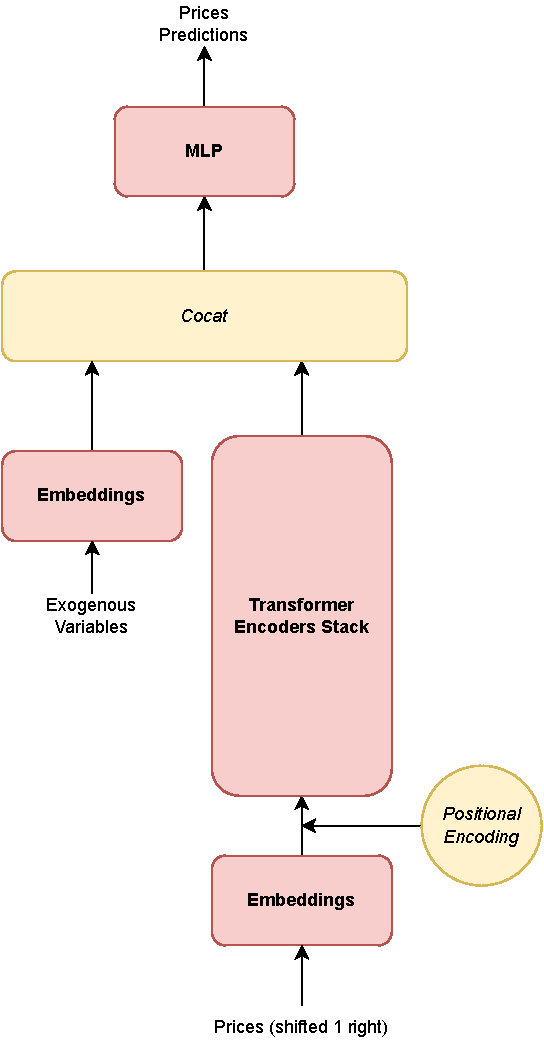
\includegraphics[width=\linewidth, height=2\linewidth]{images/model.pdf}
      \caption{Model Architecture}
      \label{fig: model architecture}
  \end{subfigure}
  \begin{subfigure}{0.49\linewidth}
    \centering
    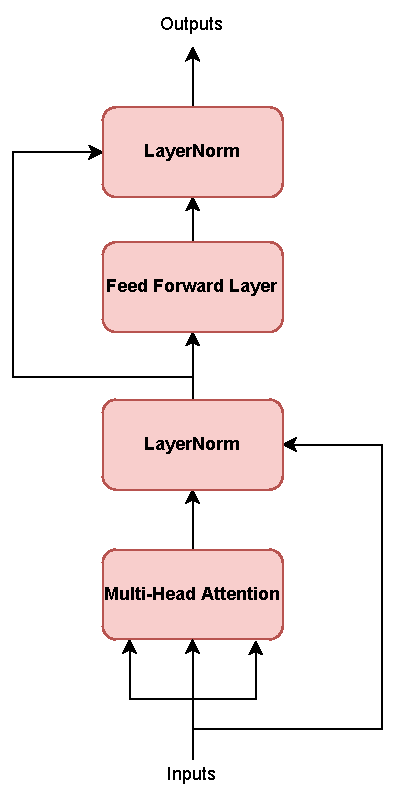
\includegraphics[width=\linewidth, height=2\linewidth]{images/transformer.pdf}
    \caption{Encoder Architecture}
    \label{fig: encoder architecture}
  \end{subfigure}
  \caption{Model and Transformer Encoder Architectures}
\end{figure}

In this case, since the objective will be to predict the 24-hour price for the next day, each day with its 24 hour will be treated as a single unit.

Next, it is also important to clarify the Embeddings layers. Even they are not really Embeddings as in NLP, this name has been adopted following the example from language models. These layers are in fact a Linear layer and a ReLU non-linearity to transform the dimension of the inputs.


\section{Case Study}

\subsection{Set Up}


\section{Conclusion}
The conclusion goes here.


\appendices
\section{Proof of the First Zonklar Equation}
Appendix one text goes here.

\section{}
Appendix two text goes here.


% use section* for acknowledgment
\section*{Acknowledgment}


The authors would like to thank...


\ifCLASSOPTIONcaptionsoff
  \newpage
\fi

\bibliographystyle{elsarticle-num}
\bibliography{main}




% that's all folks
\end{document}
